\documentclass[a4paper,12pt]{article}

\usepackage{graphicx}
\usepackage{float}

\begin{document}

% \title{THREDDS Clustering}
% \maketitle

% \setlength\parindent{0pt}

\section{Introduction}

The THREDDS project is developing middleware to bridge the gap between data providers and data users. The goal is to simplify the discovery and use of scientific data and to allow scientific publications and educational materials to reference scientific data. Due to THREDDS's lack of horizontal scalability and automatic configuration management and deployment, this service usually deals with service downtimes and time consuming configuration tasks, mainly when an intensive use is done as is usual within the scientific community (e.g. climate).

This project aims to improve the scalability of the THREDDS Data Server through the implementation of a cluster of TDS instances that are deployed in the backend and that are only visible from the outside through a reverse proxy in the frontend. This project also aims to improve the management of the TDS catalogs by partitioning the hierarchy of catalogs into multiple TDS instances that are deployed in the backend, allowing high availability of the datasets and tackling the current problem of large waiting times after performing a THREDDS reinit when publishing new catalogs.  

Instead of the classic installation and configuration of a single or multiple independent THREDDS servers, manually configured, this work presents an automatic provisioning, deployment and orchestration cluster of THREDDS servers.

\subsection{Ansible - Automatic deployment and configuration}

Ansible is a tool for automating configuration management and deployment and is used in TDS Clustering in order to automate the creation of the infrastructure.

This solution is based on Ansible playbooks, used to automate the deployment and management of the agents that conform the cluster. The playbooks are based on modules (or roles) of different backends and frontends load balancing setups and solutions. This implementation allows to configure different infrastructure and deployment setups, as more workers are easily added to the cluster by simply declaring them as Ansible variables and executing the playbooks.

\subsection{HTTP Load balancing}

The frontend load balancing system enables horizontal scalability by delegating requests to backend workers, consisting in a variable number of instances for the THREDDS server that are deployed inside Apache Tomcat containers. Through the clustering capacity of the Apache Tomcat server, in combination with the JK connector and the Apache Web Server, all HTTP features such as HTTP sessions, are available for the THREDDS cluster. This clustering also provides fault-tolerance and better reliability since if any of the workers fail another instance of the cluster can take over it.

Additonally to the Apache httpd+mod\_jk setup for the gateway, this project provides alternatives to perform the load balancing in the reverse proxy, such us HAproxy and nginx.

\subsubsection{HTTP Load balancing caveats}

In the context of HTTP load balancing, the load balancer becomes a bottleneck, since all the traffic goes through it. This is particularly problematic when large datasets are accessed by the clients, because the load balancer must perform heavy transfers of data at the kernel level, which involves a lot of overhead in data being copied from the network interface and the hard disk. This breaks the load balancer at the CPU level because of the excessive amount of work that it has to do.

\subsection{Direct Server Return}

Direct Server Return is a type of load balancing in which the load balancer routes packets to the backends without changing anything in it but the destination MAC address. The backends process the requests and answer directly to the clients, without passing through the load-balancer.

This approach do away with the bottleneck created in the load balancer by the HTTP load balancing strategy, although it requires additional low level configuration and HTTP features are not available anymore.

\section{Deployment model}

The following image provides a first overview of the deployment model.

\begin{figure}[h]
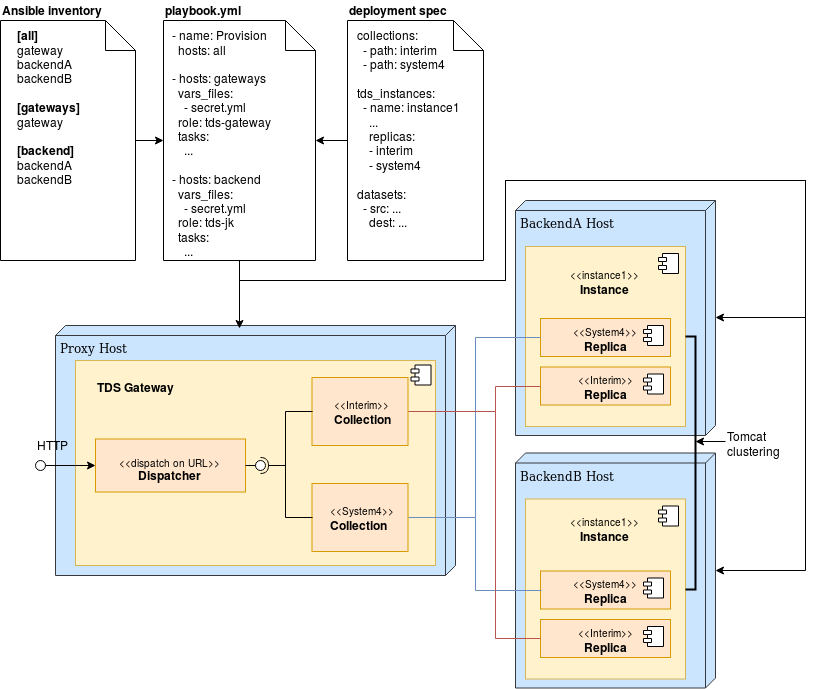
\includegraphics[width=1\textwidth]{images/overview.png}
\end{figure}

In the figure we can identify the following agents:

\begin{itemize}
\item Reverse proxy or gateway
\item Instances (THREDDS instances)
\item Collections
\item Replicas
\end{itemize}

All these elements are described in detail in the following sections.

\subsection{The gateway}

The gateway is the software that works as a reverse proxy and it is in charge of performing the load balancing, forwarding requests to the backend TDS instances deployed in Tomcat application servers. Multiple options are considered in this project to act as a gateway: httpd+mod\_jk, HAproxy, Linux Virtual Server and others.

\subsection{THREDDS instances}

Each TDS instance, or simply instance, corresponds to a Tomcat server proccess running the THREDDS web application in the backend hosts. Each host can run one or more instances. 

Each instance has the option to support any number of collections and each instance will only respond to requests targeting data available in the supported collections. This is done through the appropriate filtering of requests in the gateway.

In case of using the httpd+mod\_jk solution for the gateway, connectors of type AJP are used to connect the gateway with the instances. Usually, you only need one Connector element per gateway in the deployment, since Connector elements must reference their proxy.  Each instance can contain one or more connectors (Connector xml elements in Tomcat's server.xml).

Instances are clustered in the backend using Tomcat's clustering capabilities, which allows user session replication and in case that one of the instances become unavailable, another can take over it without any disruption of the service.

\subsection{Collections and replicas}

From an user perspective, collections are an aggrupation of catalogs and datasets. For example, the collection Interim would contain all data that belongs to ERA-Interim. Collections have no more meaning to users. However, collections allow system administrators to partition and replicate the catalog and dataset infrastructure into replicas, isolating datasets from the Interim collection from datasets of other collections. Thus, changes to the Interim collection don't have side effects on the datasets of other collections. 

From an administrator perspective, when using Apache httpd+mod\_jk in the gateway, collections are mod\_jk workers of type load balancing compunded of replicas, that is, mod\_jk balance workers. Each replica points to a tomcat instance deployed in the backend hosts that holds a copy of the contents served by the collection. Each request is routed, through the use of urimaps, to the TDS instances that support the collection in which the requested data resides.

\section{Roles and scenarios}

Ansible roles have been created to split the deployment of TDS Clustering into reutilizable parts. A user who wants to implement his specific TDS Clustering scenario has to define an Ansible inventory and playbook, and also define the variables that the Ansible roles will use to do the deployment.

\subsection{Overview of roles}

The defined Ansible roles are:

\begin{itemize}
\item[-] ansible-miniconda-role - Role to install miniconda
\item[-] virtualenv - Role to install a python virtualenv
\item[-] virtualenv-conda - Role to install a virtualenv using miniconda
\item[-] supervisord - Role to install supervisord in top of a virtualenv
\item[-] httpd - Role to install httpd from source code
\item[-] httpd-bin - Role to install httpd from system packages
\item[-] jk-gateway - Role to deploy the mod\_jk gateway in top of httpd
\item[-] tomcat - Role to deploy a tomcat server that will contain multiple instances
\item[-] tds - Role to deploy the THREDDS Data Server in tomcat instances
\item[-] tds-jk - Brigde between jk-gateway and tds
\end{itemize}

\begin{figure}[h]
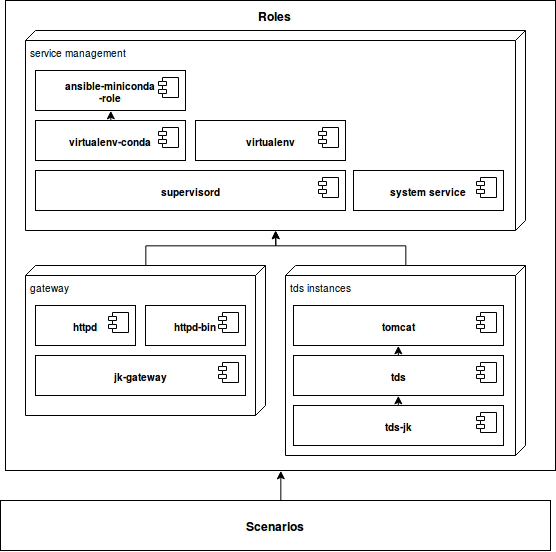
\includegraphics[width=1\textwidth]{images/roles.png}
\end{figure}

Roles are further explained in the following chapters.

\subsection{Overview of scenarios}

Scenarios are concrete use cases that make use of the available Ansible roles to do deployments with specific settings. Roles do the deployment of the minimun infrastructure for the THREDDS cluster to run and any customization must be defined in the scenarios.

Any scenario will be composed of:

\begin{itemize}
\item[-] inventory - Ansible inventory file, which defines the hosts involved in the deployment.
\item[-] main playbook - Ansible playbook that will contain two plays, one for the gateway hosts and other for the tds instances hosts, plus an optional thrird play that is in charge of the provisioning of the hosts.
\item[-] ansible.cfg - Ansible configuration file.
\item[-] user variables - Variables defined by the user that are required by the roles or that are defined to customize the deployment of the scenario.
\end{itemize}

\end{document}
